\documentclass{article}

\usepackage[margin=0.5in]{geometry}
\usepackage{enumitem}
\usepackage{graphicx}

\title{2.1 Statistics and Probability Homework Set B}
\author{}
\date{}

\begin{document}
\maketitle
\begin{enumerate}
    \item Twenty-five students have a combined average of $84$ on a test, while
        another group of twenty students have a combined average of $66$. Find
        the overall average.
        \vspace{3cm}
    \item There are $3$ blue balls and $4$ red balls in a bag. Alec
        randomly draws two balls from the bag with replacement, meaning that
        he draws one ball, replaces it, and then draws another ball. What
        is the probability that one of them is red and the other one is
        blue?
    \vspace{3cm}
    \item The faces of each of two fair dice are numbered $1$, $2$, $3$, $5$, $7$, and $8$.
        When the two dice are tossed, what is the probability that their sum will be an \underline{odd} number?
        \vspace{3cm}
    \vspace{3cm}
    % AMC 8, 2019 Problem 6
    \item There are $81$ grid points (uniformly spaced) in the square shown in the diagram below, include the points on the edges.
        Point $P$ is in the center of the square.
        Given that point $Q$ is randomly chosen among the other $80$ points, what is the probability that the line $PQ$ is a line of symmetry for the square?
        \begin{center}
            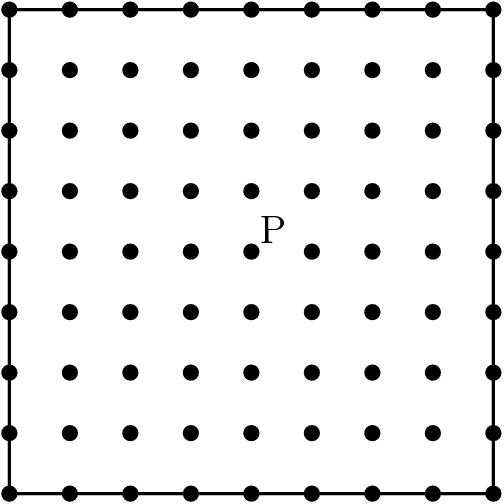
\includegraphics[scale=0.25]{grid-points.png}
        \end{center}
        \vspace{3cm}
    % AMC 8, 2007 Problem 25
    \item On the dart board shown in the figure below, the outer circle has a radius $6$ and the inner circle has radius $3$.
        Three radii divide each circle into three congruent regions, with point values shown.
        The probability that a dart will hit a given region is proportional to the area of the region.
        When two darts hit this board, the score is the sum of the point values of the regions hit.
        What is the probability that the score is odd?
        \begin{center}
            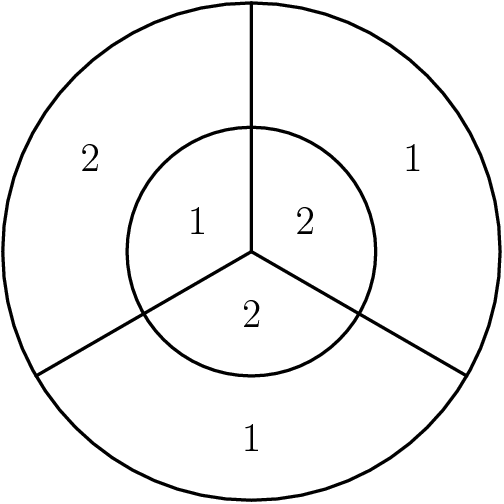
\includegraphics[scale=0.25]{dart-board.png}
        \end{center}
        \vspace{3cm}
\end{enumerate}
\end{document}
